\providecommand{\rasd}{..}
\documentclass[../RASD.tex]{subfiles}

\begin{document}
    \chapter{Formal analysis using alloy }\label{ch:formal-analysis-using-alloy}
    This section presents a possible Alloy formalization of the proposed system.
    This Alloy model illustrates the key concepts and entities that make up the system and the relationships
    between them, and is to be seen as an attempt of capturing the systems essential features.
    This model has the purpose of verifying if the properties defined for the system are possible to satisfy and if there are no constraints being violated.
    Although this model is a simplified version of the real world, it is enough to show that the model stands in the scope of the project.

    \section{Alloy Model}\label{sec:alloy-model}
        \vspace{2 mm}
        \lstinputlisting[language=alloy]{
        formal_analysis_using_alloy/alloy.als
        }
        \vspace{8 mm}

    \section{Generated World}\label{sec:generated-world}
    After running the model described above, different worlds were generated:
    \begin{figure}[H]
        \centering
        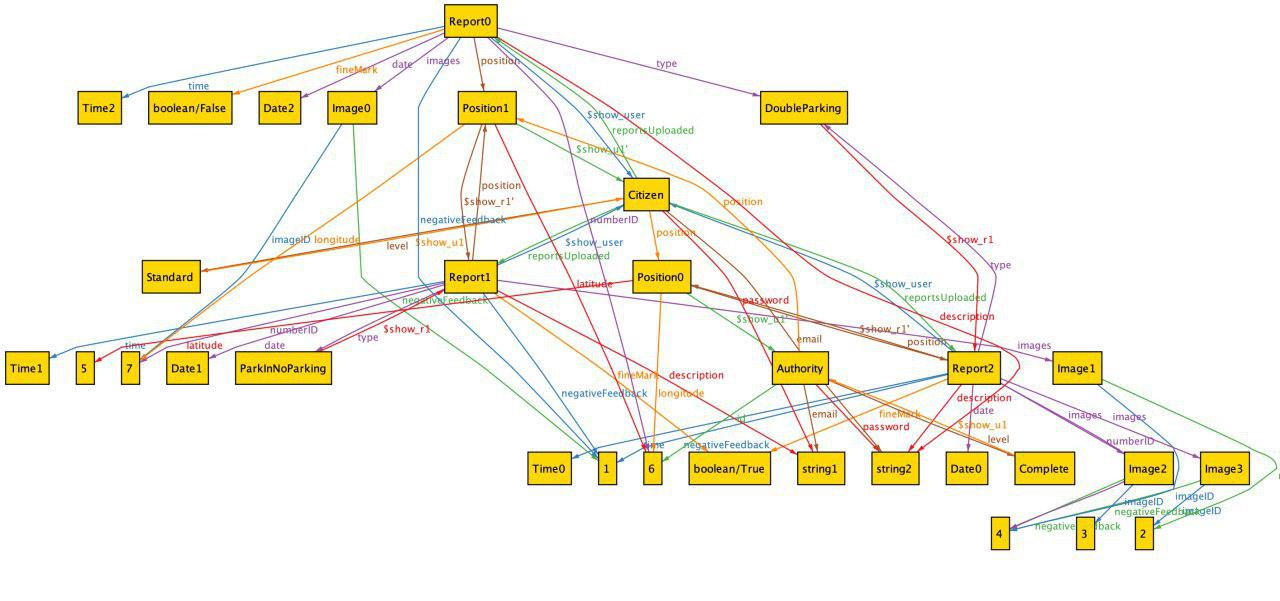
\includegraphics[scale = 0.8]{assets/generatedWorld1.png}\\[1.6 cm]
        \caption[Generated world, \textit{Alloy}]{Generated world, \textit{Alloy}}
    \end{figure}

\end{document}